Modelowanie zjawisk elektromagnetycznych realizowane jest poprzez rozwiązywanie efektywnych przybliżeń równań Maxwella dla oceny interakcji fal E-M z obiektami fizycznymi i otoczeniem. Wiele realnych problemów elektromagnetynych nie jest rozwiązywalnych na drodze analitycznej, ze względu na nieregularności gemoetryczne spotykane w strukturach czy trudne do analitycznego opisu właściwości elektromagnetyczne wykorzystywanych materiałów.


\begin{figure}[tb]
	\centering
	\begin{subfigure}{0.45\textwidth}
		
\includegraphics[width=\textwidth]{images/wstep/fdtd.png}
		\caption{}
		\label{fig:wstep-fdtd-dic}
	\end{subfigure}
	\begin{subfigure}{0.45\textwidth}
		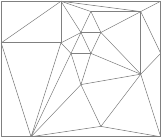
\includegraphics[width=\textwidth]{images/wstep/fem.png}
		\caption{}
		\label{fig:wstep-fem-dic}
		
	\end{subfigure}
	\caption{Porównanie siatek dyskretyzacji dla metody (a) różnic skończonych (ang. finite-difference) , (b) elementu skończonego (ang. finite-element, FEM)}
\end{figure}

Jednym ze sposobów na rozwiązywanie problemów elektromagnetycznych jest dyskretyzacja przestrzenna interesującego nas obszaru i rozwiązanie równań Maxwella dla każdego punktu dyskretyzacji\footnote{Podejście to może wymagać znaczącej mocy obliczeniowej, oraz pamięci operacyjnej wykorzystywanych komputerów. Szczególnie w symulacjach trójwymiarowych w których dwukrotne zwiększenie rozdzielczości powoduje ośmiokrotny wzrost wymaganej pamięci RAM. }. Możemy wyróżnić dwa zasadnicze sposoby wprowadzenia siatki dyskretyzacji:
\begin{itemize}
\item Metodę różnic skończonych, w której kolejne punkty obliczeniowe rozłożone są na ortogonalnej siatce równo oddalonych od siebie punktów. Ten sposób podziału obszaru obliczeniowego wiąże się z trudnościami w oddaniu nie prostokątnych kształtów geometrycznych, oraz niedokładnym odwzorowaniem obiektów, których rozmiary nie pasują do siatki dyskretyzacji. Tego typu siatkę przedstawia rysunek \ref{fig:wstep-fdtd-dic}.
\item Metodę elementu skończonego. Przygkładową siatkę dyskretyzacji przedstawia rysunek \ref{fig:wstep-fem-dic}. W przypadku metod  FEM (ang finite-element method) samo tworzenie odpowiedniej dyskretyzacji na podstawie definicji geometrii lub zdjęcia struktury może być zagadnieniem wymagającym obliczeniowo. Właściwy dobór siatki dyskretyzacji jest szczególnie ważny ze wględu na większe (w porównaniu do siatki regularnej) możliwości występowania artefaktów numerycznych.  
\item Metody w których obliczenia nie są prowadzone na dyskretnej siatce. Jak omówiona w rozdziale \ref{subart:tmm} metoda macierzy przejścia.
\end{itemize}

Wprost rozwiązując równania Maxwella poszukujemy wartości składowych pól $E$ i $H$ dla kolejnych chwil czasu. Tego typu metody określane są jako działające w dziedzinie czasu. Powszechnie wykorzystywaną metodą tego typu jest metoda różnic skończonych w dziedzinie czasu opisana szeroko w podrozdziałach \ref{subart:fdtd} - \ref{subart:borfdtd}. Największą zaletą takiego podejścia jest możliwośc zadania dowolnych prądów $J(\vec{x},t)$, przez co samam symulacja staje się sensu stricte eksperymentem numerycznym. Metody tego typu są jednak bardzo wymagające obliczeniowo, w szczególności dla symulacji trójwymiarowych dwukrotne zwiększenie gęstości siatki powoduje szesnastokrotne wydłużenie obliczeń. 

#Informacje na temat frequency domain

Wykorzystywane metody obliczeniowe można również podzielić na rozwiązujące sticte równania Maxwella, jak np. metoda FDTD, oraz metody w których numerycznemu rozwiązaniu podelga problem analitycznie uproszczony. Przykładem takiej metody jest Beam Propagation Method (BPM), w której numerycznemu rozwiązaniu podelga równanie Helmholtza.






 
